\documentclass[withoutpreface,bwprint]{cumcmthesis} %去掉封面与编号页
\title{实验报告-实验一}
\author{18340206张德龙 \\
	zhangdlong3@mail2.sysu.edu.cn
}
\date{\today}
\usepackage[cache=false]{minted}
\usepackage{diagbox}
%\usepackage{fancyhdr}
%\pagestyle{empty} 
{\renewcommand\fcolorbox[4][]{\textcolor{cyan}{\strut#4}} %屏蔽汇编语言mint的错误
\graphicspath{{figure/}}

\let\algorithm\relax  
\let\endalgorithm\relax 
\usepackage[linesnumbered,ruled,lined]{algorithm2e}
\usepackage{algpseudocode}  
\renewcommand{\algorithmicrequire}{\textbf{Input:}}   
\renewcommand{\algorithmicensure}{\textbf{Output:}}   
\SetKwFor{For}{for}{do}{endfor}
\newcommand{\ret}{\textbf{return}}   

\makeatletter
\newenvironment{breakablealgorithm}
{% \begin{breakablealgorithm}
	\begin{center}
		\refstepcounter{algorithm}% New algorithm
		\hrule height.8pt depth0pt \kern2pt% \@fs@pre for \@fs@ruled
		\renewcommand{\caption}[2][\relax]{% Make a new \caption
			{\raggedright\textbf{\ALG@name~\thealgorithm} ##2\par}%
			\ifx\relax##1\relax % #1 is \relax
			\addcontentsline{loa}{algorithm}{\protect\numberline{\thealgorithm}##2}%
			\else % #1 is not \relax
			\addcontentsline{loa}{algorithm}{\protect\numberline{\thealgorithm}##1}%
			\fi
			\kern2pt\hrule\kern2pt
		}
	}{% \end{breakablealgorithm}
		\kern2pt\hrule\relax% \@fs@post for \@fs@ruled
	\end{center}
}
\makeatother

\newcounter{Emp}[subsubsection]	% 设置计数器
\newcommand{\kuohao}{\addtocounter{Emp}{1} \noindent (\theEmp)}

\usepackage{amssymb}% http://ctan.org/pkg/amssymb
\usepackage{pifont}% http://ctan.org/pkg/pifont
\newcommand{\cmark}{\ding{51}}%
\newcommand{\xmark}{\ding{55}}%

\usepackage{threeparttable}

\begin{document}
\maketitle
\begin{abstract}
 
 在本次实验中,我们小组实现了模拟退火算法和遗传算法,并且进行了多个对比实验。模拟退火实验结果显示了区间翻转邻域操作在寻找TSP解上具有一定的优越性;并且结果显示,采取单一邻域操作的效果比不上结合先验知识,依据概率选取邻域操作的混合邻域操作。 %hc
 \keywords{模拟退火 \quad 遗传算法 \quad 混合邻域}
\end{abstract}

\section{导言}

在TSPLIB\footnote{http://comopt.ifi.uni-heidelberg.de/software/TSPLIB95/}中选一个大于100个城市数的TSP问题,采用模拟退火算法和遗传算法求解。模拟退火算法要求如下:
\begin{enumerate}
\item 采用多种邻域操作的局部搜索local search策略求解;
\item 在局部搜索策略的基础上,加入模拟退火simulated annealing策略,并比较两者效果;
\item 要求求得的解不要超过最优值的10%,并能够提供可视化。
\end{enumerate}


遗传算法要求如下:
\begin{enumerate}
\item 设计较好的交叉操作,并且引入多种局部搜索操作;
\item 和之前的模拟退火算法(采用相同的局部搜索操作)进行比较;
\item 得出设计高效遗传算法的一些经验,并比较单点搜索和多点搜索的优缺点。
\end{enumerate}
	

\section{实验过程-模拟退火算法}

\subsection{多种邻域操作的局部搜索}
局部搜索算法是在一组可行解的基础上,在当前解的领域内进行局部搜索产生新的可行解的过程。局部搜索是解决最优化问题的一种启发式算法。对于某些计算起来非常复杂的最优化问题,比如各种NP完全问题,要找到最优解需要的时间随问题规模呈指数增长,因此诞生了各种启发式算法来退而求其次寻找次优解,是一种近似算法(Approximate  algorithm),基于以时间换精度的思想。局部搜索就是其中的一种方法。
\subsubsection{多种邻域操作}

参考文献\cite{1}中的多种启发式邻域操作,本次实验中我们小组所使用的邻域操作有:

\kuohao 两点交换:

本邻域操作的动作为将路径中的随机两点进行交换操作:
\begin{figure}[H]
	\centering
	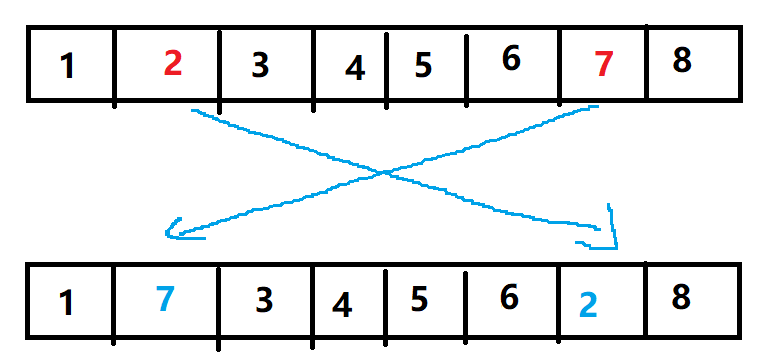
\includegraphics[width=0.5\linewidth]{swap}
	\caption{两点交换}
\end{figure}

\kuohao 区间翻转:

本邻域操作的动作为将路径中的随机区间进行翻转操作:
\begin{figure}[H]
	\centering
	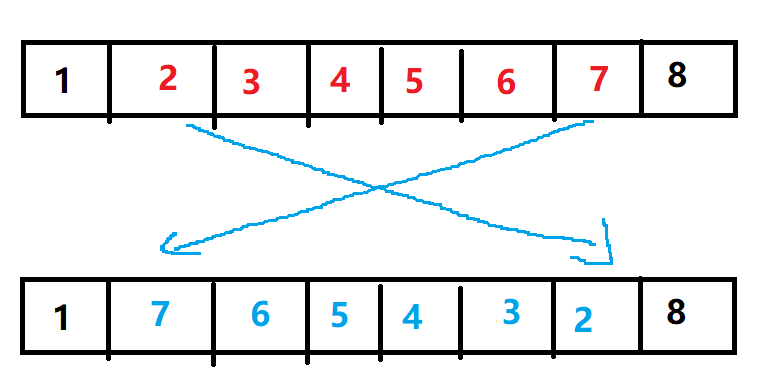
\includegraphics[width=0.5\linewidth]{reverse}
	\caption{区间翻转}
\end{figure}
\kuohao 随机置顶:

本邻域操作的动作为随机选取路径中的两点并顶置,其余点顺序不变:
\begin{figure}[H]
	\centering
	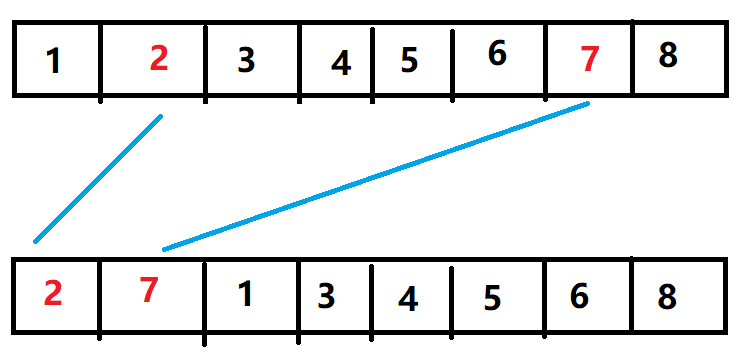
\includegraphics[width=0.5\linewidth]{rd_top}
	\caption{随机置顶}
\end{figure}

\subsubsection{实验设置及结果}
随机初始化解,采用早停法,为了与模拟退火对标,局部搜索同样设置内循环,循环次数为解长度的10倍,早停法容忍次数设置为50次。对不同的邻域操作进行实验,取5次随机运行后所得的最好解、最差解、平均值、标准差作为指标显示如下,百分比为相对于最优解的百分比:
\begin{table}[H]
\centering
\caption{局部搜索实验结果}
\begin{tabular}{|c|c|c|c|c|}
\hline
\textbf{局部搜索} & \textbf{最好解}     & \textbf{最差解}     & \textbf{平均值}     & \textbf{标准差}    \\ \hline
\textbf{两点交换} & 45.38\%          & 66.42\%          & 58.15\%          & 8.26\%          \\ \hline
\textbf{区间翻转} & \textbf{13.47\%} & \textbf{19.41\%} & \textbf{15.55\%} & \textbf{2.23\%} \\ \hline
\textbf{随机置顶} & 149.45\%         & 181.80\%         & 159.88\%         & 12.36\%         \\ \hline
\end{tabular}
\end{table}
从结果可以得到,采用区间翻转邻域操作的局部搜索效果最优,最优解与目前最优值的差值达到了13.47\%,其余邻域操作的效果相比区间翻转操作有大幅度的下降。绘制区间翻转的最优解如下所示:
\begin{figure}[H]
		\centering
		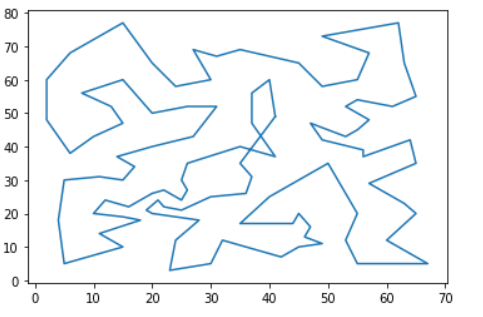
\includegraphics[width=0.5\linewidth]{ls_b}
		\caption{采用区间翻转邻域操作的局部搜索最优解}
\end{figure}


\subsection{模拟退火}
	模拟退火相比局部搜索优越的地方在于其能够通过接受劣解来达到最终获得更优解的效果。其接受劣解的概率由Metropolis准则决定,通过劣解与目前最优解目标值的距离以及当前温度来决定接收劣解的概率,模拟退火的流程图和伪代码图\ref{flow}所示。
	\begin{figure}[htbp]]
		\centering
		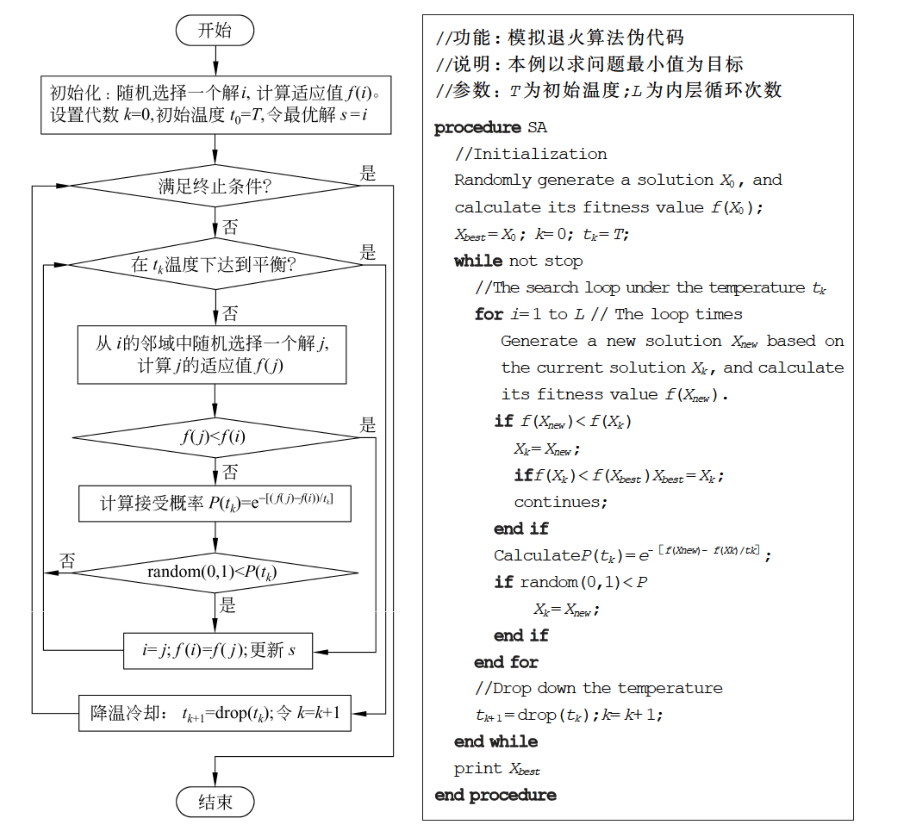
\includegraphics[width=1\linewidth]{sa_flow}
		\caption{模拟退火的流程图和伪代码}
		\label{flow}
	\end{figure}
		
\subsubsection{实验设置及结果}
随机初始化解,采用早停法,设置内循环次数为解长度的10倍,早停法容忍次数设置为50次。对不同的邻域操作进行实验,取5次随机运行后所得的最好解、最差解、平均值、标准差作为指标显示如下,百分比为相对于最优解的百分比:
\begin{table}[H]
\centering
\caption{模拟退火实验结果}
\label{sa}
\begin{tabular}{|c|c|c|c|c|}
\hline
\textbf{模拟退火} & \textbf{最好解}    & \textbf{最差解}     & \textbf{平均值}     & \textbf{标准差}    \\ \hline
\textbf{两点交换} & 13.66\%         & 25.04\%          & 17.97\%          & \textbf{3.90\%} \\ \hline
\textbf{区间翻转} & \textbf{6.08\%} & \textbf{29.28\%} & \textbf{16.06\%} & 8.10\%          \\ \hline
\textbf{随机置顶} & 119.33\%        & 141.59\%         & 125.93\%         & 8.15\%          \\ \hline
\end{tabular}
\end{table}
从结果可以得到,与局部搜索结果类似,采用区间翻转邻域操作的效果最优,最优解与目前最优值的差值达到了6.08\%,其余邻域操作的效果相比区间翻转操作有些微的下降,但是相比与局部搜索可得,模拟退火使得效果有了明显的提升。绘制区间翻转的最优解如下所示:
\begin{figure}[H]
		\centering
		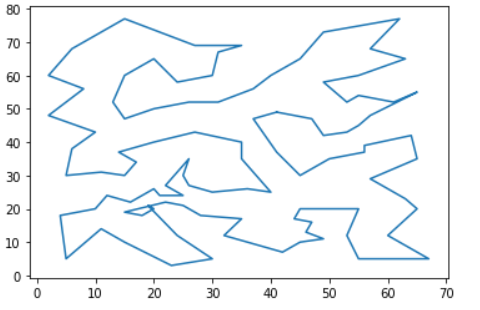
\includegraphics[width=0.5\linewidth]{sa_b}
		\caption{采用区间翻转邻域操作的模拟退火最优解}
\end{figure}


\subsection{改进:混合邻域操作}
	根据上述结果可得,采用区间翻转的效果相比使用其他的邻域操作效果更好,但是考虑到仅一种邻域操作对解的搜索强度不如随机选取邻域操作,因此结合先验知识,采用混合邻域操作,选取两点交换、区间翻转、随机置顶邻域操作的概率为[0.01, 0.98, 0.01],随机选取可以简单地通过numpy库的choice函数进行实现:
	\begin{lstlisting}[language=python]
		func = np.random.choice([self.neighbour_swap, self.neighbour_two_opt_swap, self.neighbour_two_h_opt_swap], p=[0.01, 0.98, 0.01])
	\end{lstlisting}
	
	LS代表局部搜索、SA代表模拟退火,实验结果对比为:
\begin{table}[H]
\centering
\caption{实验结果}
\label{all}
\begin{tabular}{|c|c|c|c|c|}
\hline
\textbf{方案}                            & \textbf{最好解}    & \textbf{最差解}     & \textbf{平均值}     & \textbf{标准差}    \\ \hline
\textbf{两点交换-LS} & 45.38\%  & 66.42\%  & 58.15\%  & 8.26\%  \\ \hline
\textbf{区间翻转-LS} & 13.47\%  & 19.41\%  & 15.55\%  & 2.23\%  \\ \hline
\textbf{随机置顶-LS} & 149.45\% & 181.80\% & 159.88\% & 12.36\% \\ \hline
\multicolumn{1}{|l|}{\textbf{混合邻域-LS}} & 11.25\%         & 15.52\%          & 13.63\%          & \textbf{1.52\%} \\ \hline
\textbf{两点交换-SA} & 13.66\%  & 25.04\%  & 17.97\%  & 3.90\%  \\ \hline
\textbf{区间翻转-SA} & 6.08\%   & 29.28\%  & 16.06\%  & 8.10\%  \\ \hline
\textbf{随机置顶-SA} & 119.33\% & 141.59\% & 125.93\% & 8.15\%  \\ \hline
\multicolumn{1}{|l|}{\textbf{混合邻域-SA}} & \textbf{4.15\%} & \textbf{16.48\%} & \textbf{11.24\%} & 4.76\%          \\ \hline
\end{tabular}
\end{table}

   从结果可以得到,采用混合邻域操作的模拟退火算法效果最优,达到了4.15\%。采用混合邻域操作后,不管是局部搜索还是模拟退火算法的效果都有显著的提升,显示了混合邻域操作的优越性。绘制最终的得到的最优解如下所示:
   \begin{figure}[H]
   		\centering
   		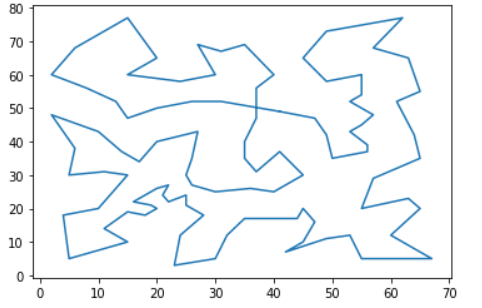
\includegraphics[width=0.5\linewidth]{sa_br}
   		\caption{最终得到的最优解}
   \end{figure}

	
\section{结论-模拟退火算法}
	在本次实验中,我们小组实现了局部搜索和模拟退火算法,并且就多种邻域操作进行了对比。实验结果显示了区间翻转邻域操作在寻找TSP解上具有一定的优越性;并且结果显示,采取单一邻域操作的效果比不上结合先验知识,依据概率选取邻域操作的混合邻域操作;并且混合邻域操作对于局部搜索和模拟退火两个算法的效果都有提升。
	

\section{实验过程-遗传算法}
遗传算法是用于解决最优化的搜索算法,借鉴了进化生物学中的一些现象而发展起来,这些现象包括遗传、突变、自然选择以及杂交。现代遗传算法把每个个体抽象为染色体,使种群向更好的解进化。一般包括以下几个环节:选择、交配池中交叉、变异、交叉产生新后代、新选择,然后一直循环直到满足终止条件。算法框架如下
\begin{figure}[H]
		\centering
		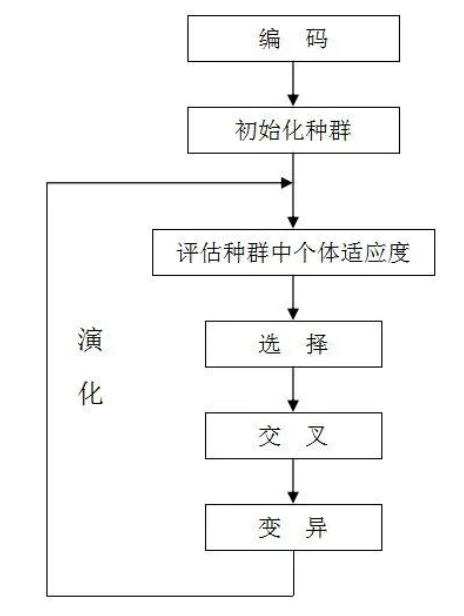
\includegraphics[width=0.5\linewidth]{algo}
		\caption{遗传算法流程}
\end{figure}
本次实验中,我们小组从各个环节进行设计,遗传算法取得比模拟退火算法更优的结果。
\subsection{个体的编码}
tsp问题中,设有$N$个城市,视每个城市为一个数字,那么$1$到$N-1$的数字的乱序组合就是一个可能的解,假设这个组合是$ABC...N$,那么去到城市$A$后下一步去到城市$B$,再去到城市$C$...最后城市$N$再去到城市$A$,就得到了一条回路,这是tsp问题的一个可能最优解。
\subsection{贪婪算法的遗传池初始化}
传统遗传算法完全从随机的初始种群开始,所以需要很长的时间才能交配出正确解。但在tsp问题中,采用贪婪方式进行初始化,已经能够得到一个不错的个体。这些个体前半部分的基因组合十分贴近最优解,在循环的一开始就引入这些基因片段无疑是十分有利的。 \par
算法简要描述如下,对于$N$个点,任选1个点$A$,然后,在剩余$N-1$个点中找到距离$A$最近的点$B$,那么就认为取到点$A$后向点$B$走。之后将$A$从$N$个点剔除,然后寻找点$B$在剩余$N-2$个点中距离最近的点$C$,以此类推。这样就得到一个$ABC...N$的初始个体,由于每次起始点A都是随机选取的,遗传池中的个体也各有不同,保证了一定的随机性。
\par
贪婪算法虽然有效,但也存在性能的问题,以上描述的算法是$O(n^2)$的,为了找到每个点最近的点,需要遍历所有其他点。为此我们引入了阈值,使得算法早些停下来,在算法中,如果找到两个点之间的距离小于$d$,那就视为找到该点最近的点,经测试,d取为横纵坐标最大跨度的1\%效果最好。
\subsection{PMX交叉}
对于个体的交叉方式,我们使用PMX算法,这个算法对于每个个体都寻找随机的一段,然后将两端交换得到两个后代,之后建立起两端之间的数字关联,在后代中补充因为交换缺少的数字,如下图所示:
\begin{figure}[H]
		\centering
		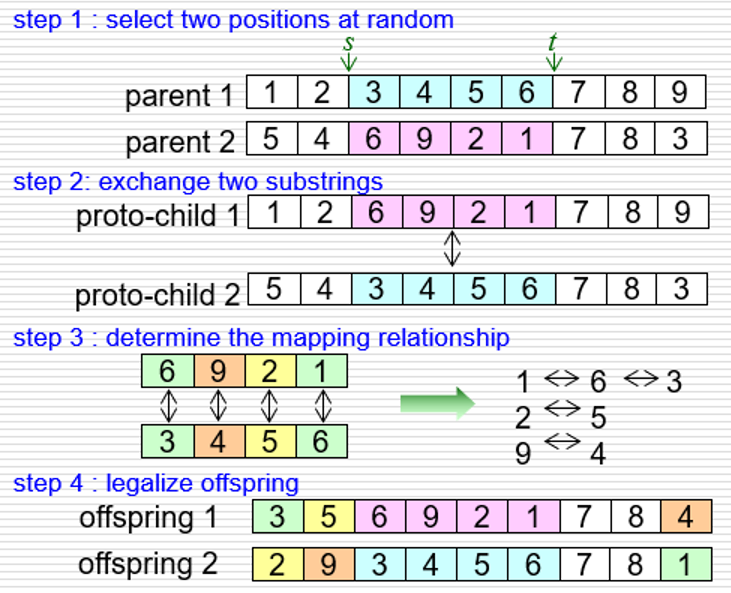
\includegraphics[width=0.5\linewidth]{PMX}
		\caption{PMX算法图解}
\end{figure}
这对于tsp问题是最优异的一种交叉方式,这是因为它保留了完整的基因片段。在贪婪初始化的过程中,我们得到了很好的起始基因,这种交叉方式恰好能够保留这些基因。所以这种交叉方式很适合我们的遗传算法,在实际的实现中,我们对这个算法进行了简单的改进,比起随机选择两段基因,我们先随机选出一段基因,然后在另一个个体中找到开头相同的另一端基因。这样做,替换的基因大概率是相近的,能够最大概率的用好的基因替换坏的基因。
\subsection{变异方式}
常用的变异方式也是前面提到的局部搜索,但我们最终在遗传算法中使用更有效的方式。这种方式是随机顶置的变体。每次变异中,随机选取一个点$A$,然后寻找距离$A$最近的点$B$,直接把$B$插入到点$A$的后方。采用这种方法最大的好处是结果不会变坏,选取的$B$有两种情况:第一种是$B$本身就在$A$的后方,此时变异个体与原个体一致;第二种是$B$原本不在$A$的后方,设原本个体为$AC...DBE$,变异后个体变为$ABC...DE$,那么路径中减少了$AC$、$DB$、$BE$增加了$AB$、$BC$、$DE$,由于三角形性质$DB + BE \geq DE$,并且$AC \geq AB$,只要$BC$较小,进行这样的变异就总是更好的。
\subsection{选择}
常见的选择方式有轮盘赌选择、Boltzmann选择、繁殖池选择等方法。但经过测试这些方法的效果都差不多,要使遗传算法效果最好,核心还是放在交叉和变异上。所以最终我们采用随机选择法,我们维护大小为$15$的繁殖池,然后每次交叉任意选择两个个体,重复20次,取最好的个体。变异的选择也类似,重复变异20次,选择其中最好的后代。繁殖池每次都保留最好的15个个体,需要注意将父代从池中提出,不然繁殖池会高度相似,个体失去多样性
\section{结果分析-遗传算法}
遗传算法也选择eil101问题进行求解,迭代5000次。
\begin{figure}[H]
		\centering
		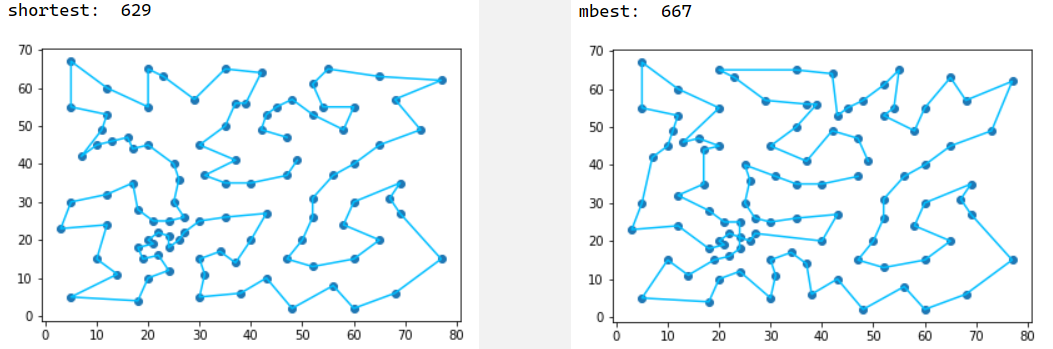
\includegraphics[width=1\linewidth]{compare}
		\caption{eil101最优解和我们的解对比}
\end{figure}
此时得到的最好解与最优解相差6\%,虽然略弱于模拟退火算法。但在运行时间上,遗传算法只需要30s,而模拟退火算法需要10min,使用遗传算法远远快于遗传算法。使用遗传算法得到更优的效果,这是各个环节都优化组合的结果。\par
本算法还有可以改进的地方,在课堂分享中,有的小组采用多种变异方式混合的方法,取得了更好的结果,这是十分值得尝试和探索的思路。

\section{结论-遗传算法}
	在本次实验中,我们对tsp问题进行了模拟退火算法和遗传算法求解的探索。在遗传算法的设计中,我们设计了较好的交叉操作,并测试了多种局部搜索操作,采用了最优的变异方式。与模拟退火算法比较过程中,我们发现,精心设计的遗传算法能够以极快的速度取得接近模拟退火算法准确率的可接受解。\par
	多点搜索对比单点搜索有一个很大的优势,多点搜索可以更快的速度收敛。因为多点搜索总是能很快的试错,然后经过反复随机搜索,探索更广的搜索空间,找到其中一个最优解,这点单点搜索比不上。但单点搜索允许更细致的搜索,单点搜索虽然比较慢,但是只要给出足够的时间,就能得到更精确的解。我们的实验中也验证了这一点:模拟退火算法速度慢,但是得到更精确的解。\par
	经过这次实验,我们更加深入理解了模拟退火算法和遗传算法,也对于经典tsp问题积累了一些经验。
	
   

%\section{错误检测与恢复实验结果截图}
%\begin{figure}[H]
%	\centering
%	\includegraphics[width=1\linewidth]{errinput}
%	\caption{错误样例输入}
%\end{figure}
%\subsection{实验结果}
%\begin{figure}[H]
%	\centering
%	\includegraphics[width=1\linewidth]{cuowu}
%	\caption{错误检测与恢复实验结果}
%\end{figure}
%\begin{appendices}
%\end{appendices}
%
\begin{thebibliography}{99}
	\bibitem{1} Lin S . Computer solutions of the traveling salesman problem[J]. Bell Labs Technical Journal, 1965, 44(10):2245-2269.
	
	\bibitem{2} Yang W H, Mathur K, Ballou R H. Stochastic vehicle routing problem with restocking[J]. Transportation Science, 2000, 34(1): 99-11
	
	\bibitem{3} Potvin J Y, Rousseau J M. An exchange heuristic for routeing problems with time windows[J]. Journal of the Operational Research Society, 1995, 46(12): 1433-1446.

\end{thebibliography}

\end{document}